\subsection{Nabomatricer}
En anden mulighed for at repræsentere en graf er ved brug af nabomatricer. Nabomatricer er bedre, når grafen har mange kanter.\\
En nabomatrice kan beskrives som en $N=m X m$ matrice, hvor $m$ er afhængig af knudemængden $V=\{v_0, v_1, \ldots, v_m\}$. Hvis man har en simpel graf, $G=(V,E)$, vil matricen være en nul-1 matrice, da en simpel graf kan kun have en kant mellem to knuder. Når der er en kant mellem to  vilkårlig knuder, $(v_i,v_j)$,  vil den få notationen 1, hvis der derimod ikke er en kant vil får den notation 0. \\

Det kan også skrives som \\

\begin{equation}
\begin{Bmatrix} 
	 \hspace{0.3cm}\textrm{1 hvis} \hspace{0.3cm}\{v_i,v_j\} \hspace{0.2cm} \textrm{har en kant i grafen} \hspace{0.2cm} G \\
	 \textrm{0 ellers} \\
	\end{Bmatrix}
\end{equation}

\begin{figure}[H]
  \centering
  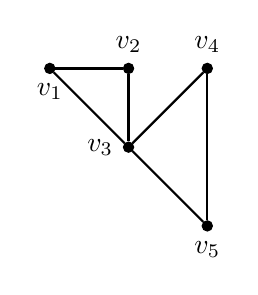
\begin{tikzpicture}
  \tikzset{enclosed/.style={draw, circle, inner sep=0pt, minimum size=.13cm, fill=black}}
  	\node[enclosed] at (0,2) (v1) [label=below:\(v_1\)] {};
    \node[enclosed] at (1,2) (v2) [label=above:\(v_2\)] {};
    \node[enclosed] at (1,1) (v3) [label=left:\(v_3\)] {};
    \node[enclosed] at (2,2) (v4) [label=above:\(v_4\)] {};
    \node[enclosed] at (2,0) (v5) [label=below:\(v_5\)] {};
    
	\path[thick] (v1) edge node {} (v2);
	\path[thick] (v1) edge node {} (v3);
	\path[thick] (v2) edge node {} (v3);
	\path[thick] (v4) edge node {} (v3);
	\path[thick] (v5) edge node {} (v3);   
	\path[thick] (v4) edge node {} (v5); 

  \end{tikzpicture}
  \caption{Ikke-orienteret, simpel graf.}
  \label{fig:stm}
\end{figure}

  \label{fig:simpelgraf}
\end{figure}

Nabo natricen nedenfor bruger rækkefølgen $v_1$,$v_2$,$v_3$,$v_4$,$v_5$
\begin{equation}
	\begin{bmatrix}
		0&1&1&0&0 \\
		1&0&1&0&0 \\
		1&1&0&1&1 \\
		0&0&1&0&1 \\
		0&0&1&1&0 \\
	\end{bmatrix}
\end{equation}

	

